\begin{center}
    \section*{\myul{Wärmestrahlung}}
\end{center}

\begin{tikzpicture}[remember picture, overlay]

% ---- ERSTE REIHE: Am Seitenursprung starten
\setlength{\rowheight}{64mm} % Erste Reihenhöhe: 20mm

    % A1) Erste Kachel am Seitenursprung ausrichten
    \setlength{\cellwidth}{88mm} % Breite einstellen
    \Tile{A1}{([xshift=10mm,yshift=-18mm]current page.north west)}{\cellwidth}{\rowheight}
        {
            \vspace{-\TileSep}
            \begin{minipage}{0.39\cellwidth-\TileSep}
                \centering
                \titlebf{1. Hauptsatz}\\ \vspace{-2mm}
                \begin{equation*}
                    \dot W + \dot Q + \Phi = \dot U
                \end{equation*}
                \vspace{-1.5mm}
            \end{minipage}%
            \vrule
            \begin{minipage}{0.59\cellwidth-\TileSep}
                \centering
                \titlebf{Konvektive Übertragung}\\ \vspace{-2.5mm}
                \begin{equation*}
                    \dot Q_{12} = \alpha\,A\,(T_1 - T_2)
                \end{equation*}
                \vspace{-1.5mm}
            \end{minipage}%
            \vspace{1mm}
            \rule{\dimexpr\cellwidth-2\TileSep}{0.5pt} \\ \vspace{0.5mm}
            \titlebf{Definition des Raumwinkels} \\ \vspace{3mm}
            \begin{minipage}{0.50\cellwidth-\TileSep}
                \centering
                \begin{equation*}
                    \text{d}\Omega = \frac{\text{d}A}{r^2} = \sin(\vartheta)\,\text{d}\vartheta\,\text{d}\varphi
                \end{equation*}
            \end{minipage}%
            \begin{minipage}{0.48\cellwidth-\TileSep}
                \centering
                \vspace{1mm}
                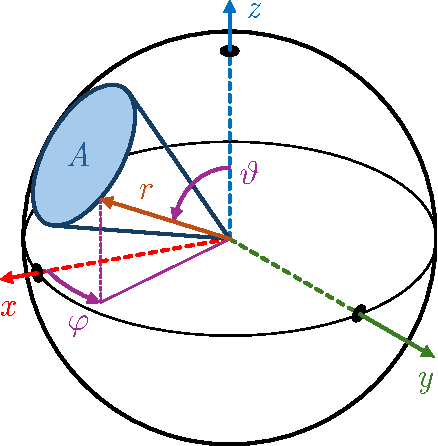
\includegraphics[height=32mm]{images/raumwinkel.pdf}
            \end{minipage}
        }{0}{1}{1}{0} % Kanten: unten & rechts

    % B1) Zweite Kachel rechts anbauen
    \setlength{\cellwidth}{102mm} % Breite einstellen
    \Tile{B1}{(A1.north east)}{\cellwidth}{\rowheight}
        {
            \vspace{-\TileSep}
            \titlebf{Sichtfaktor}\\ \vspace{2mm}
            \begin{minipage}{0.5\cellwidth-\TileSep}
                \centering
                \titlerm{Allgemein}\vspace{-1mm}
                \begin{equation*}
                    F_{i\rightarrow j} = \frac{\Phi_{i\rightarrow j}}{\Phi_i} \leq 1
                \end{equation*}
                \begin{equation*}
                    A_i\,F_{i\rightarrow j} = A_j\,F_{j\rightarrow i}
                \end{equation*}
                \vspace{-1mm}
                \begin{equation*}
                    \sum\limits_j F_{i\rightarrow j} = 1
                \end{equation*}
                \vspace{1mm} \\
                \titlerm{Differenziell}\vspace{-1mm}
                \begin{equation*}
                    \text{d}F_{i\rightarrow j}~\text{d}A_i = \text{d}F_{j\rightarrow i}~\text{d}A_j
                \end{equation*}
                \vspace{-2mm}
                \begin{equation*}
                    = \frac{\text{d}A_i\,\cos(\vartheta_i)~\text{d}A_j\,\cos(\vartheta_j)}{\pi\,r^2}
                \end{equation*}
                \vspace{-0.5mm}
            \end{minipage}%
            \vrule
            \begin{minipage}{0.5\cellwidth-\TileSep}
                \centering
                \vspace{-5mm}
                \begin{equation*}
                    H_i = \frac{K_i}{A_i} = \sum\limits_i M_i
                \end{equation*}
                \begin{equation*}
                    E_{i\rightarrow j} = F_{j\rightarrow i}~H_i
                \end{equation*}
                \rule{\dimexpr\textwidth-2\TileSep}{0.5pt} \\ \vspace{0.5mm}
                \titlerm{Raumwinkel-Näherung} \\ \vspace{0.5mm}
                ($A_\text{i}$ \&  $A_\text{j}$ eben, $\vartheta_i = \vartheta_j = 0$)
                \begin{equation*}
                    \Omega_j \approx \frac{A_j}{r_{ij}^2} \stackrel{!}{<} \text{0,2}
                \end{equation*}
                \vspace{-5.5mm} \\
                \hspace{45mm}{\color{RedOrange}sfn()} \\
                \vspace{-5.5mm}
                \begin{equation*}
                    F_{i\rightarrow j} = \frac{\Omega_j}{\pi} \approx \frac{A_j}{\pi\,r_{ij}^2}
                \end{equation*}
            \end{minipage}
        }{0}{0}{1}{0} % Kante: unten

% ---- ZWEITE REIHE: Unten anbauen
\setlength{\rowheight}{24mm}

    % A2) Erste Kachel unten anbauen
    \setlength{\cellwidth}{90mm}
    \Tile{A2}{(A1.south west)}{\cellwidth}{\rowheight}
        {
            \titlerm{Differenzieller Ansatz}\\ \vspace{-2mm}
            \begin{equation*}
                F_{i\rightarrow j} = \frac{\int_{A_j} \int_{A_i} \frac{M_i}{\pi\,r^2}\,\cos(\vartheta_i)\,\cos(\vartheta_j)\,\text{d}A_i\,\text{d}A_j}{\int_{A_i} M_i\,\text{d}A_i}
            \end{equation*}
        }{0}{1}{1}{0}

    % B2) Zweite Kachel rechts anbauen
    \setlength{\cellwidth}{100mm}
    \Tile{B2}{(A2.north east)}{\cellwidth}{\rowheight}
        {
            \titlerm{Gekreuzte Fäden}\\ \vspace{-2mm}
            \begin{equation*}
                F_{1\rightarrow 2} = \frac{\sum L_\text{(Gekreuzte Fäden)} - \sum L_\text{(Ungekreuzte Fäden)}}{\sum L_\text{(Emittierende Linie)}}
            \end{equation*}
        }{0}{0}{1}{0}

% ---- DRITTE REIHE: Unten anbauen
\setlength{\rowheight}{42mm}

    % A3) Erste Kachel unten anbauen
    \setlength{\cellwidth}{190mm}
    \Tile{A3}{(A2.south west)}{\cellwidth}{\rowheight}
        {
            \titlebf{Zusammenfassung}\\ \vspace{2mm}
            \begin{tabular}{Sc|Sc|Sc}
                {\color{Blue}Elementarfläche} $\rightarrow$ {\color{Blue}Elementarfläche} & $\displaystyle\text{d}F_{\text{d}1\rightarrow \text{d}2} = \frac{\cos(\vartheta_1)\,\cos(\vartheta_2)}{\pi\,r_{12}^2}\,\text{d}A_2$ & $\displaystyle\text{d}F_{\text{d}1\rightarrow \text{d}2}\,\text{d}A_1 = \text{d}F_{\text{d}2\rightarrow \text{d}1}\,\text{d}A_2$ \\ \hline
                {\color{Blue}Elementarfläche} $\rightarrow$ {\color{OliveGreen}Endliche Fläche} & $\displaystyle F_{\text{d}1\rightarrow 2} = \int_{A_2}\frac{\cos(\vartheta_1)\,\cos(\vartheta_2)}{\pi\,r_{12}^2}\,\text{d}A_2$ & $\displaystyle F_{\text{d}1\rightarrow \text{d}2}\,\text{d}A_1 = \text{d}F_{\text{d}2\rightarrow \text{d}1}\,A_2$ \\ \hline
                {\color{OliveGreen}Endliche Fläche} $\rightarrow$ {\color{OliveGreen}Endliche Fläche} & $\displaystyle F_{1\rightarrow 2} = \frac{1}{A_1}\,\int_{A_1} \int_{A_2} \frac{\cos(\vartheta_1)\,\cos(\vartheta_2)}{\pi\,r_{12}^2}\,\text{d}A_2\,\text{d}A_1$ & $\displaystyle F_{\text{d}1\rightarrow \text{d}2}\,A_1 = F_{\text{d}2\rightarrow \text{d}1}\,A_2$
            \end{tabular}
        }{0}{0}{1}{0}

% ---- VIERTE REIHE: Unten anbauen
\setlength{\rowheight}{50mm}

    % X4) EIGENES FELD für die Zeilen-Überschrift
    \Tile{X4}{(A3.south west)}{190mm}{9mm}
        {
            \vspace{1mm}
            \titlebf{Wärmeübertragung durch Strahlung} \\
        }{0}{0}{0}{0}

    % A4) Erste Kachel unten anbauen
    \setlength{\cellwidth}{95mm}
    \Tile{A4}{(X4.south west)}{\cellwidth}{\rowheight}
        {
            \vspace{-\TileSep}
            \titlerm{Flächenspezifische Strahlungsleistung}\\ \vspace{2mm}
            \begin{minipage}{0.5\cellwidth-\TileSep}
                \centering
                Allgemein:
                \begin{equation*}
                    M = \frac{\text{d}\Phi}{\text{d}A_1} = L\,\int\cos(\vartheta)\,\text{d}\Omega
                \end{equation*}
                konst. $\Rightarrow$ homogen
                \rule{\dimexpr\textwidth-2\TileSep}{0.5pt} \\ \vspace{0.5mm}
                Kirchhoff I:
                \begin{equation*}
                    M_\text{S} = \frac{M_i}{\alpha_i} = \text{konst.}
                \end{equation*}
            \end{minipage}%
            \vline
            \begin{minipage}{0.5\cellwidth-\TileSep}
                \centering
                Lambert'scher Strahler:
            \end{minipage}
        }{0}{1}{1}{0}

    % B4) Erste Kachel unten anbauen
    \setlength{\cellwidth}{95mm}
    \Tile{B4}{(A4.north east)}{\cellwidth}{\rowheight}
        {
            \vspace{-\TileSep}
            \titlerm{Flächenspezifische Strahlungsleistung}\\ \vspace{2mm}
            
        }{0}{0}{1}{0}

\end{tikzpicture}